\documentclass{article}
\usepackage[utf8]{inputenc}
\usepackage{authblk}
\usepackage{setspace}
\usepackage[margin=1.25in]{geometry}
\usepackage{graphicx}
\graphicspath{ {./figures/} }
\usepackage{amsmath,amssymb,amsfonts}
\usepackage{booktabs}
\usepackage{natbib}
\usepackage{hyperref}
\hypersetup{colorlinks=true, linkcolor=blue, citecolor=blue, urlcolor=blue}

\title{\textbf{Recurrent Neural Networks versus HAR for Five-Day-Ahead Volatility Forecasts of Equities and Bitcoin}}
\author[1]{hypoq autonomous research harness}
\affil[1]{Hypothesis $\times$ Quant}
\date{\today}
\onehalfspacing

\begin{document}
\maketitle

\begin{abstract}
\noindent \textbf{Hypothesis:} $H_0$: an LSTM and the HAR benchmark have equal expected QLIKE loss for the 5-day-ahead variance; $H_1$: the LSTM has lower loss \\
\textbf{Data:} Daily OHLC of the S\&P 500 and Bitcoin; S\&P 500 test 2023-01-03 to 2026-10-16 (951 days); Bitcoin test 2023-01-01 to 2026-10-20 (1,389 days) \\
\textbf{Method:} Garman--Klass variance, HAR on log variance, LSTM on 22-day windows with early stopping and 5 seeds, chronological split at 2023-01-01, one-sided DM test with HAC errors, Bonferroni $\alpha=0.025$ \\
\textbf{Results:} S\&P 500: QLIKE HAR 0.2263 vs LSTM 0.2348 (DM $p=0.742$); Bitcoin: QLIKE HAR 0.2727 vs LSTM 0.2361 (DM $p=0.000$). Decision: \textbf{INCONCLUSIVE}
\end{abstract}

\section{Design}
The target is the log mean Garman--Klass variance of the next five sessions. HAR regresses it on the current, weekly and monthly log variance \citep{corsi2009simple}; the LSTM sees the same information as 22-day windows. Both receive the same log-normal bias correction when converted to variance. Training labels that overlap the test period are purged.

\section{Results}
\begin{table}[h!]
\centering
\caption{Out-of-sample forecast loss (lower is better) and one-sided Diebold--Mariano test, H$_1$: LSTM better}
\begin{tabular}{lcccccc}
\toprule
Asset & QLIKE HAR & QLIKE LSTM & MSE-log HAR & MSE-log LSTM & DM $t$ & $p$ \\
\midrule
S\&P 500 & 0.2263 & 0.2348 & 0.3836 & 0.3902 & -0.65 & 0.7417 \\
Bitcoin & 0.2727 & 0.2361 & 0.4525 & 0.4146 & 3.76 & 0.0001 \\
\bottomrule
\end{tabular}
\end{table}


\begin{figure}[h!]
\centering
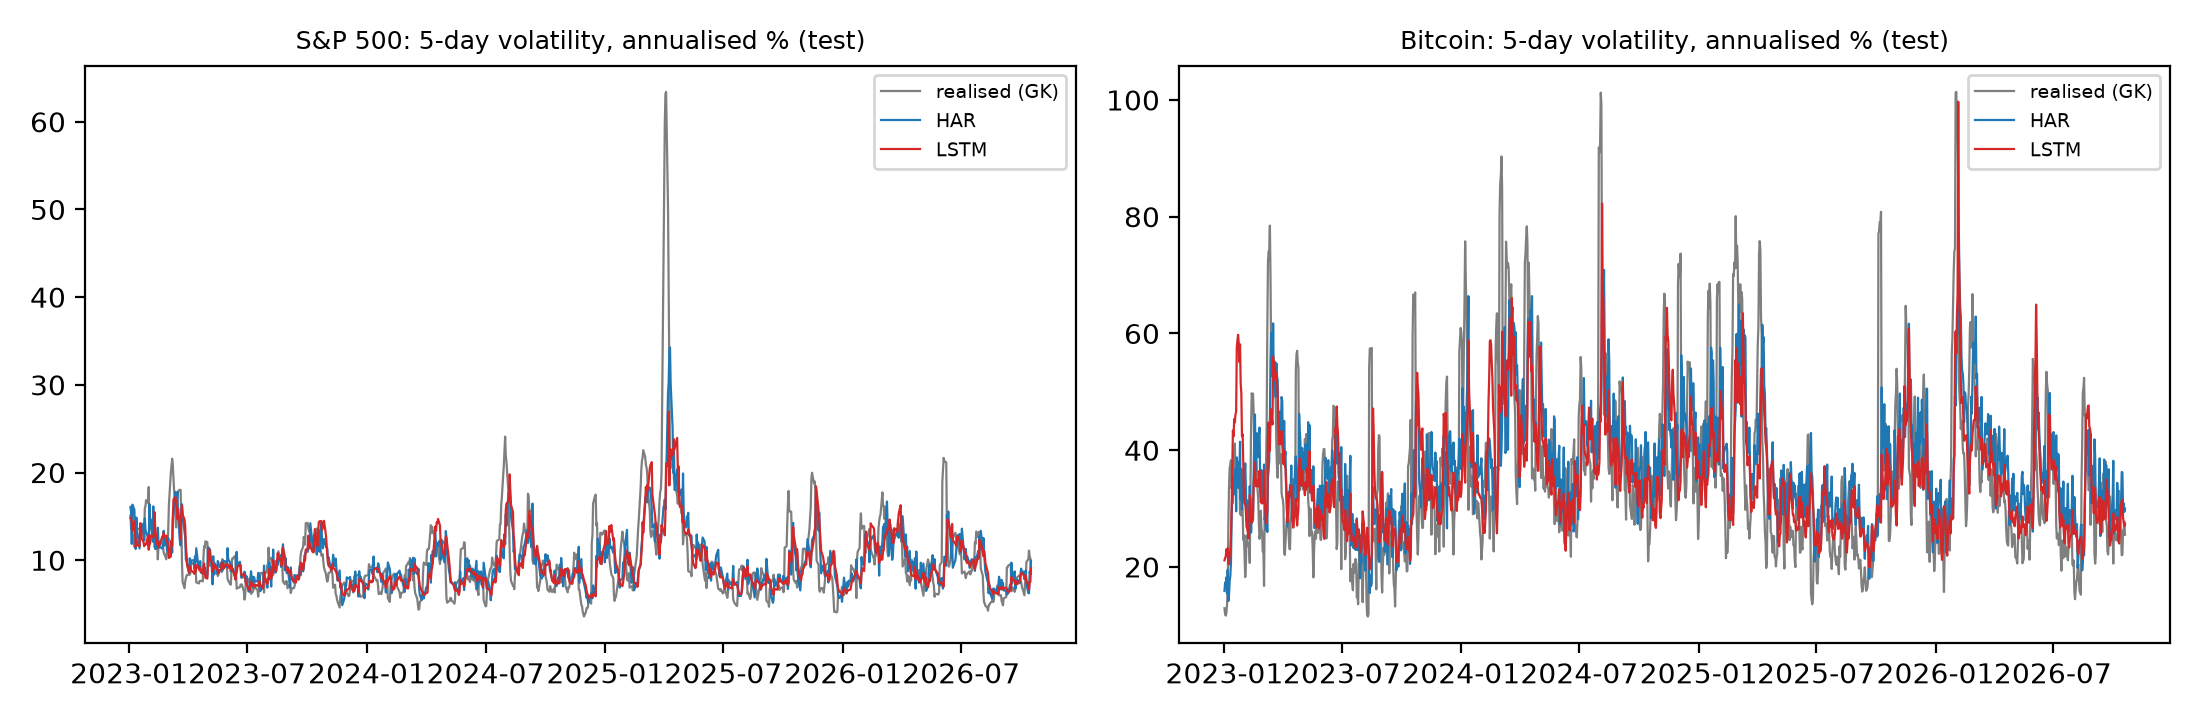
\includegraphics[width=\textwidth]{fig1_volatility_forecasts.png}
\caption{Test-period forecasts.}
\end{figure}

\section{Limitations}
Garman--Klass from daily bars is a noisy proxy for realised variance; one chronological split is used rather than rolling re-estimation; the network is small and its hyper-parameters were not tuned on the test period.


\bibliographystyle{plainnat}
\bibliography{references}

\end{document}
